%%%%%%%%%%%%%%%%%%%%%%%%%%%%%%%%%%%%%%%%%%%%%%%%%%%%%%%%%%%%%%%%%%%%%%%%%%
% policy2, v2plot.pdf, v9plot
% annotation?
\begin{figure*}[tbp!]
\vspace{-2mm}
\centering
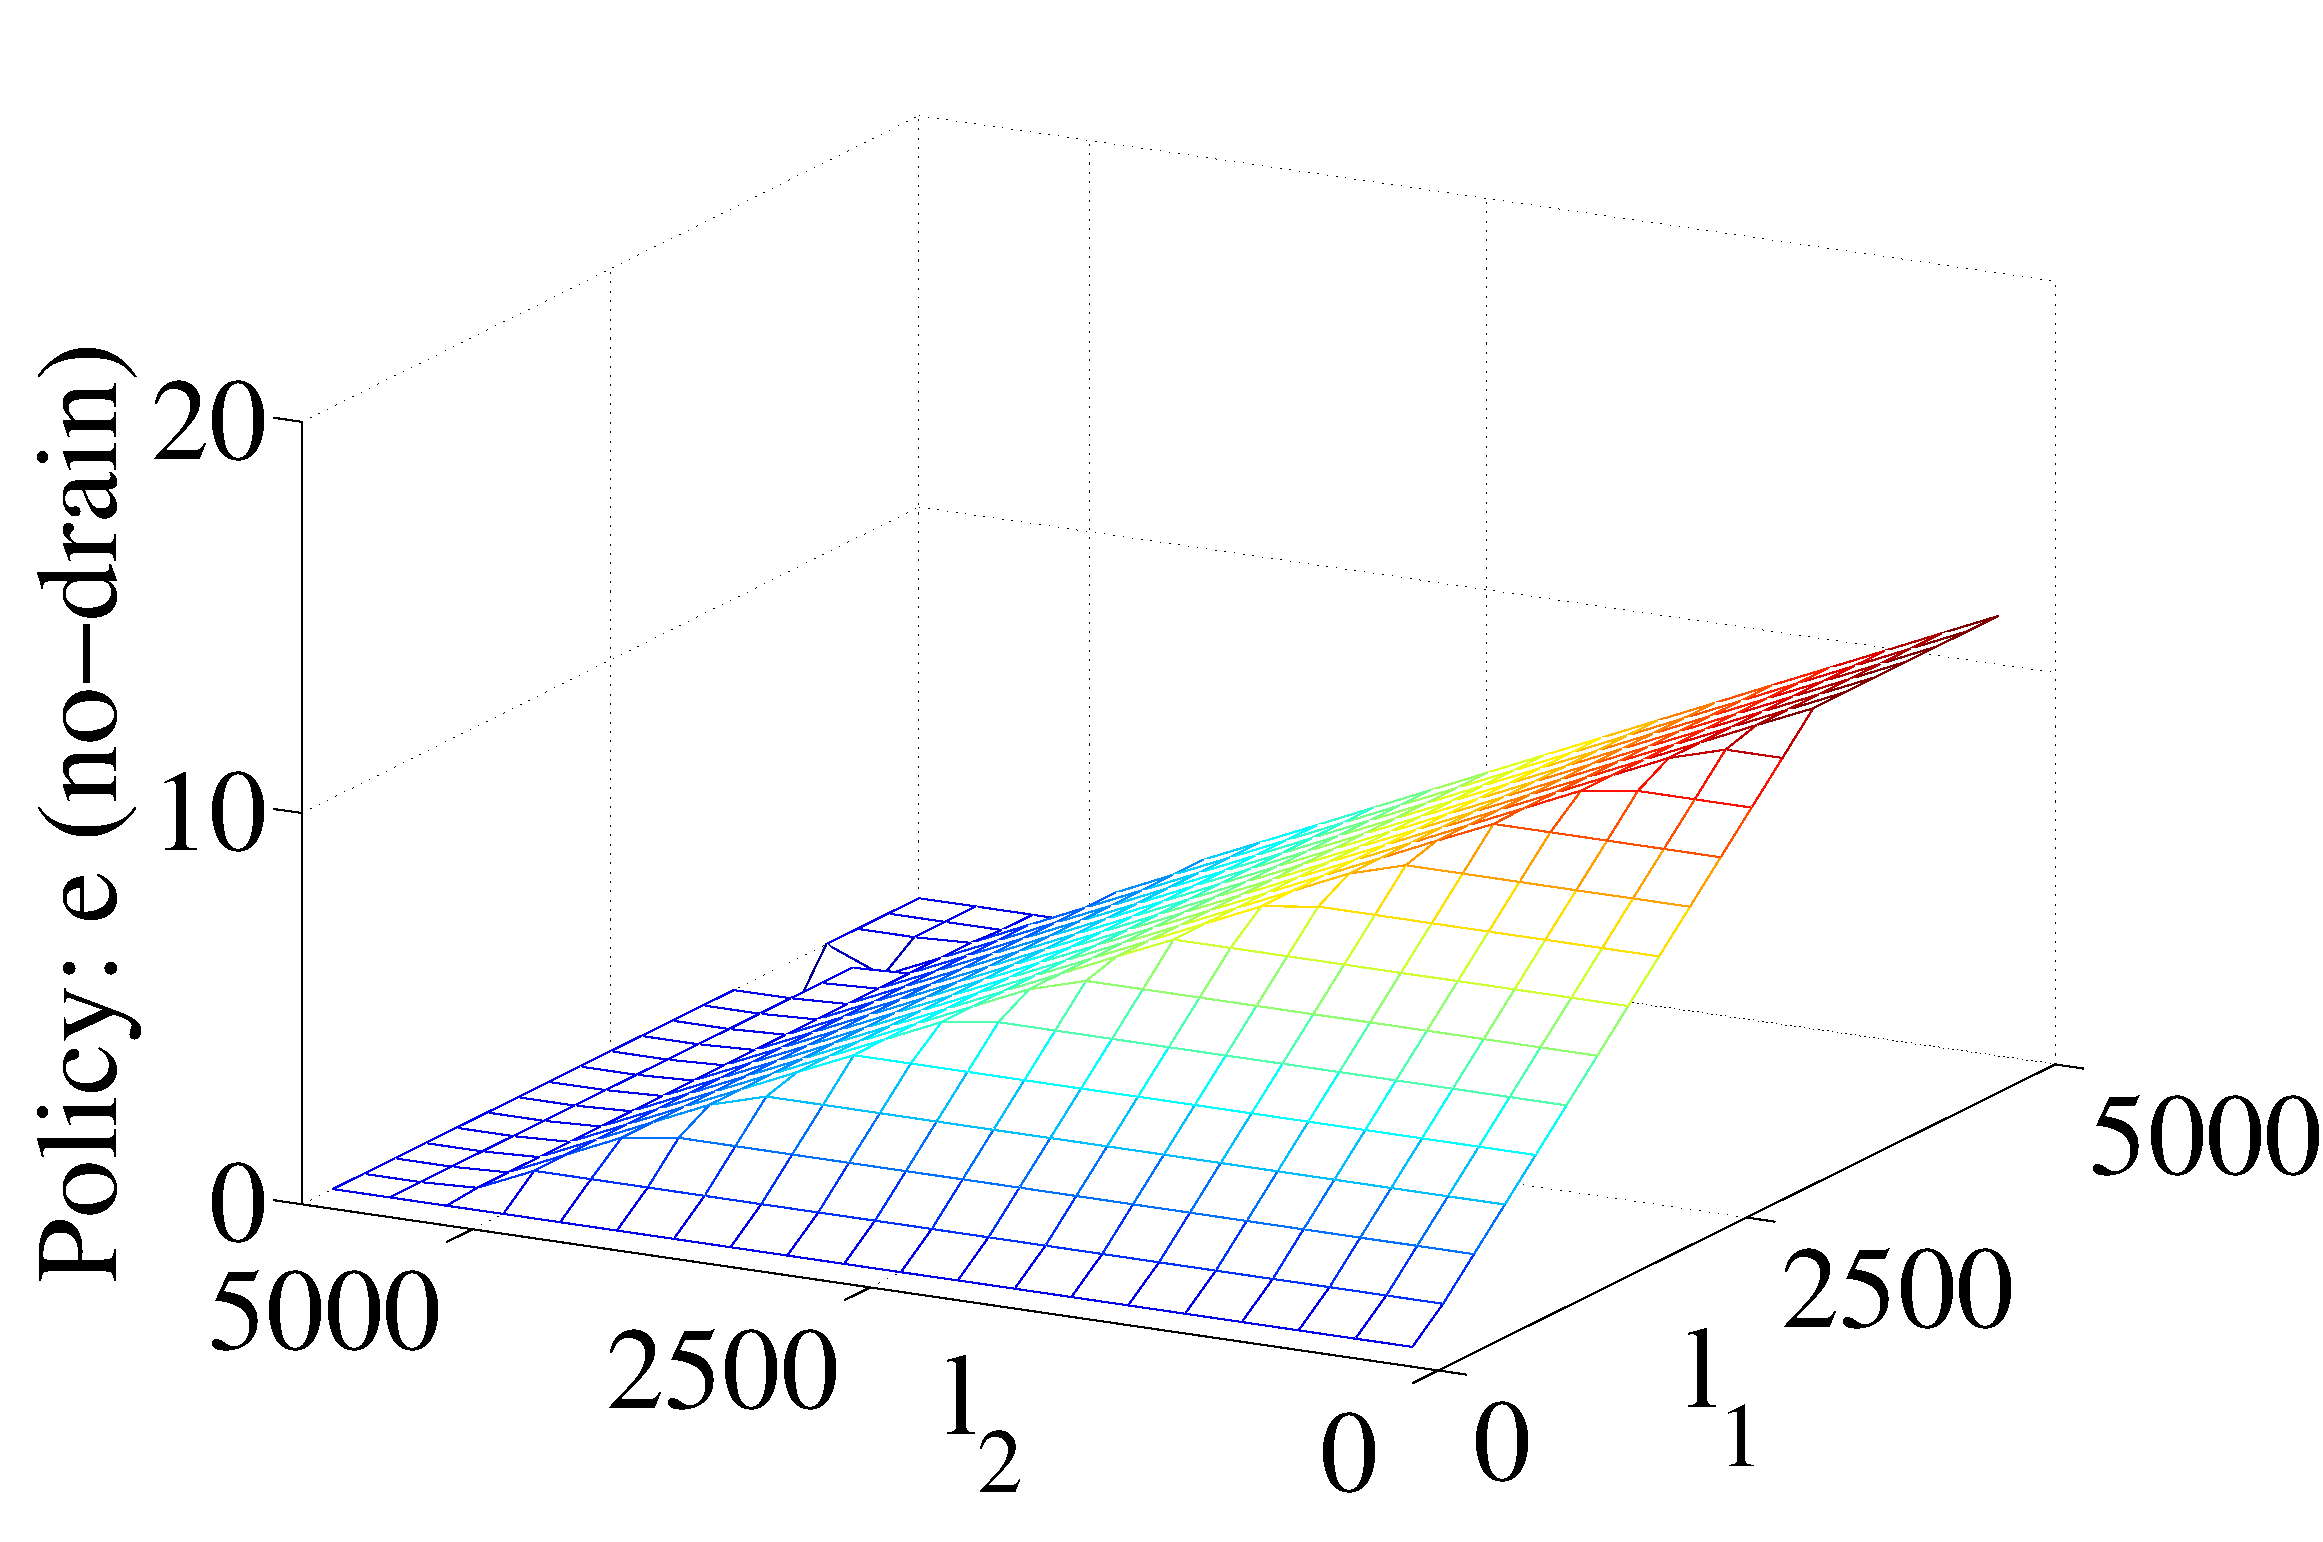
\includegraphics[width=0.3\textwidth]{new_pics/policy-iteration2-3.pdf}
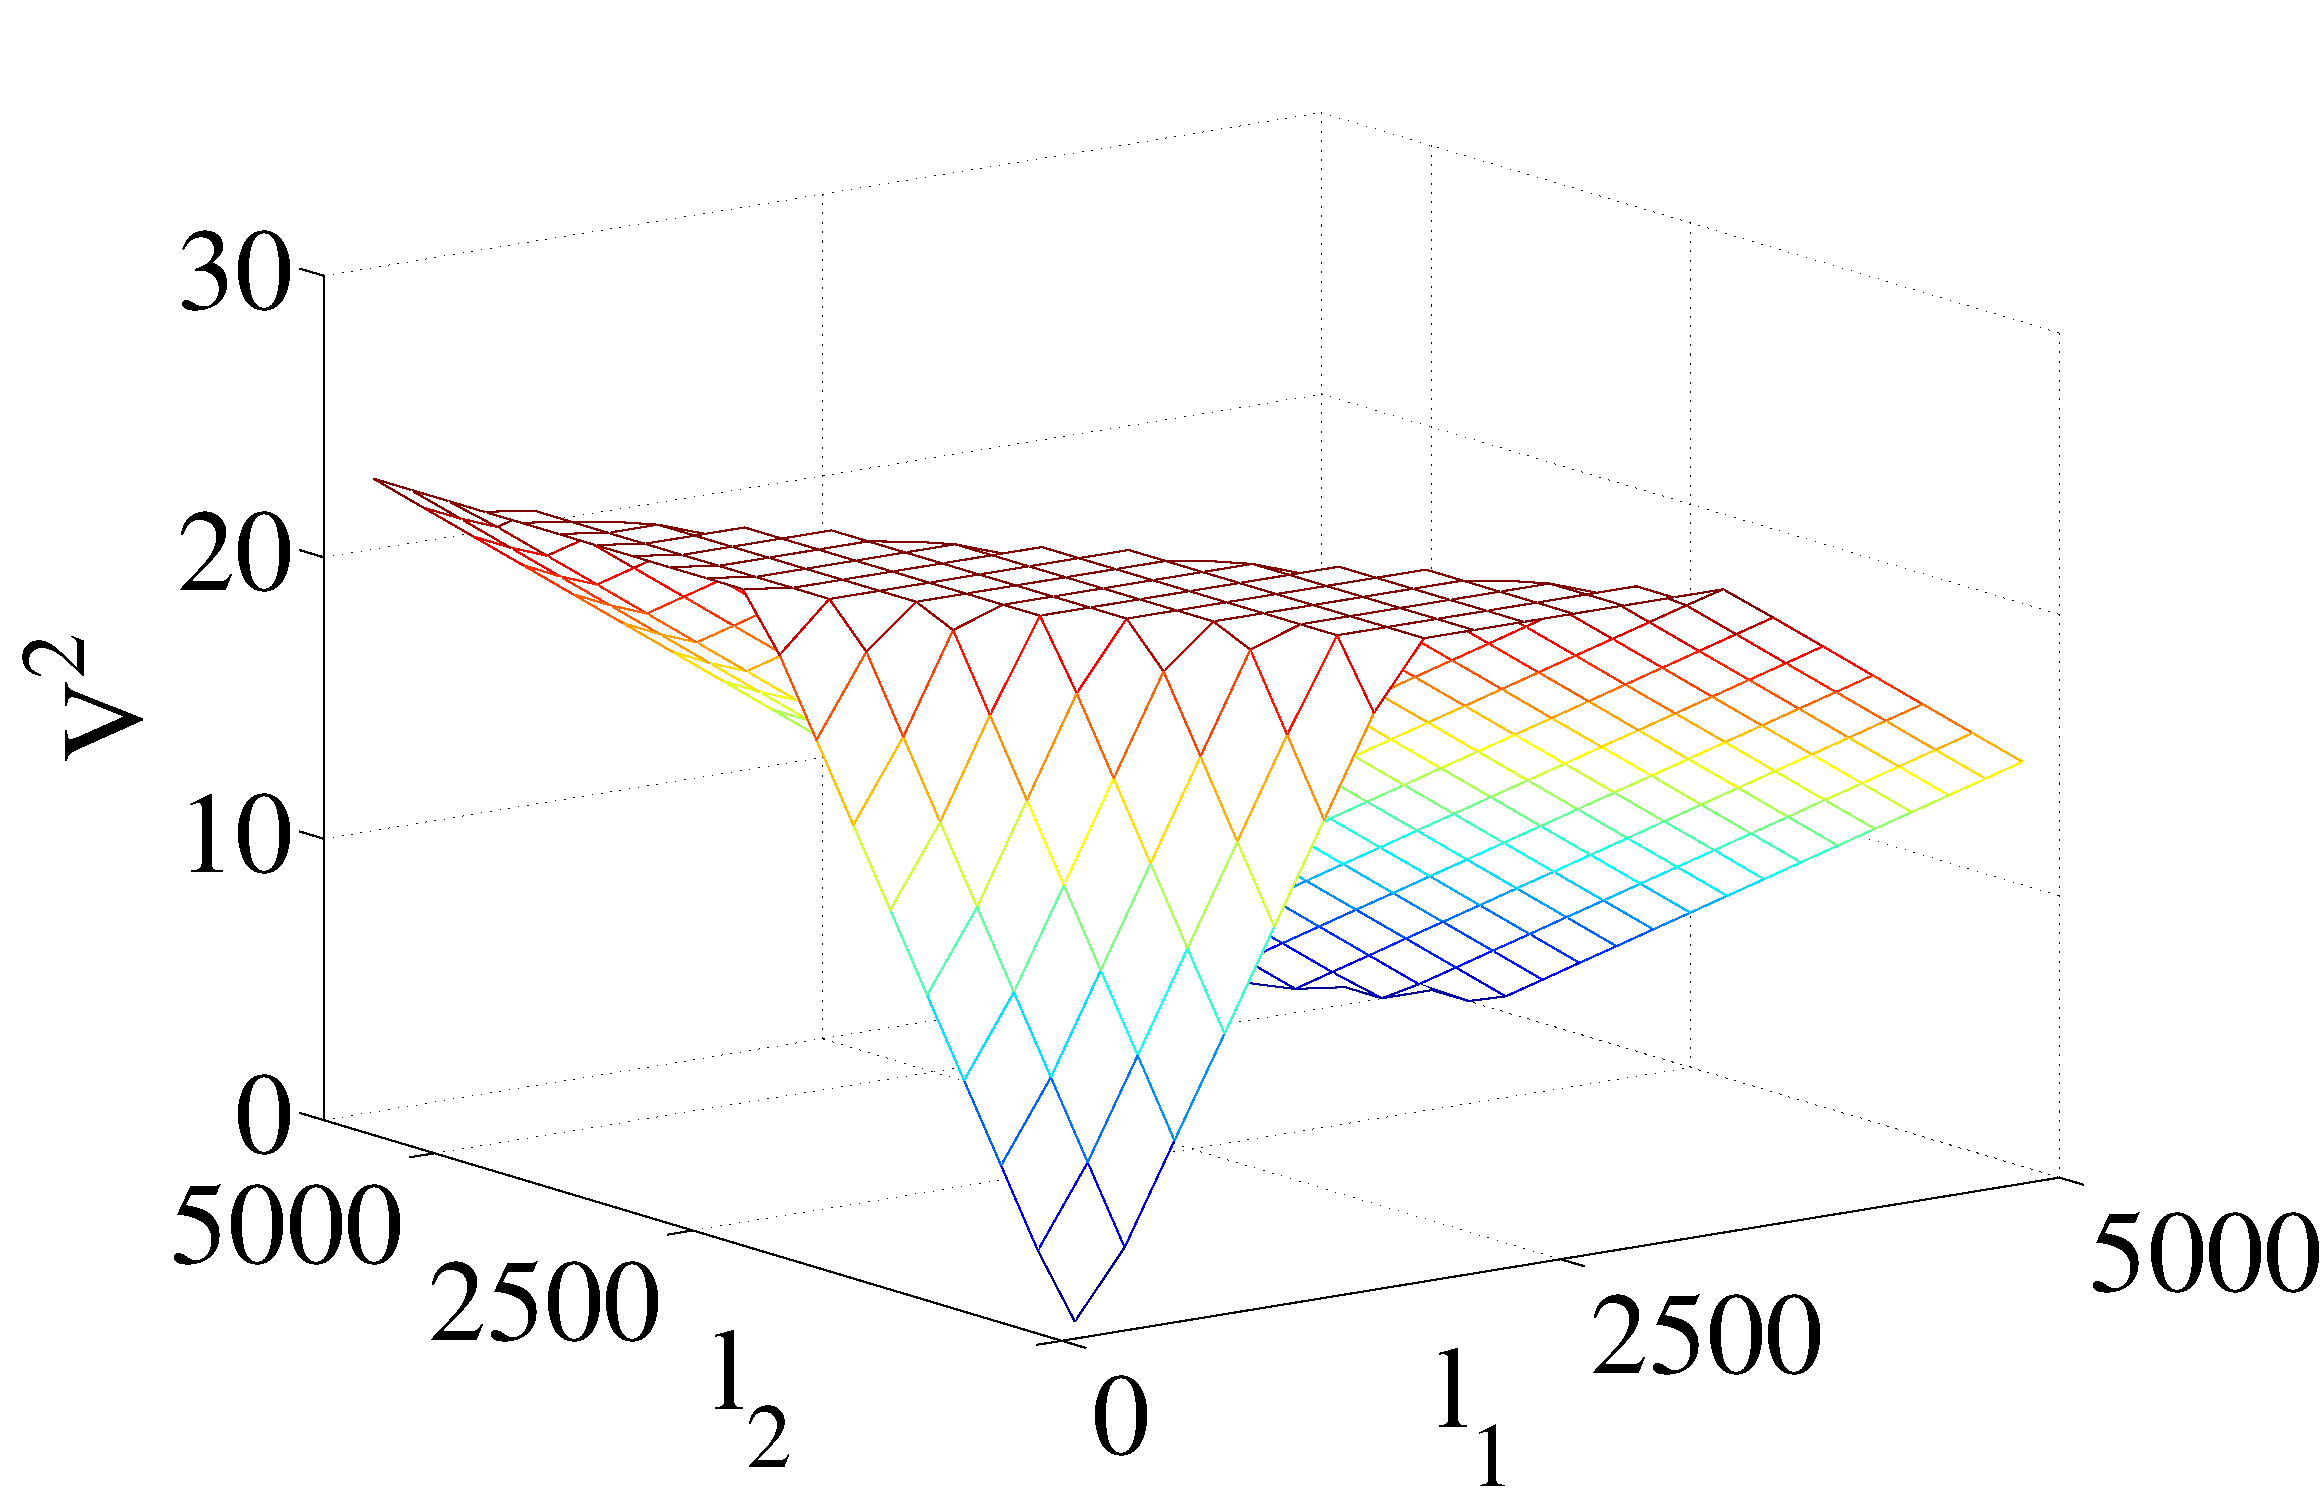
\includegraphics[width=0.3\textwidth]{new_pics/V2.pdf}
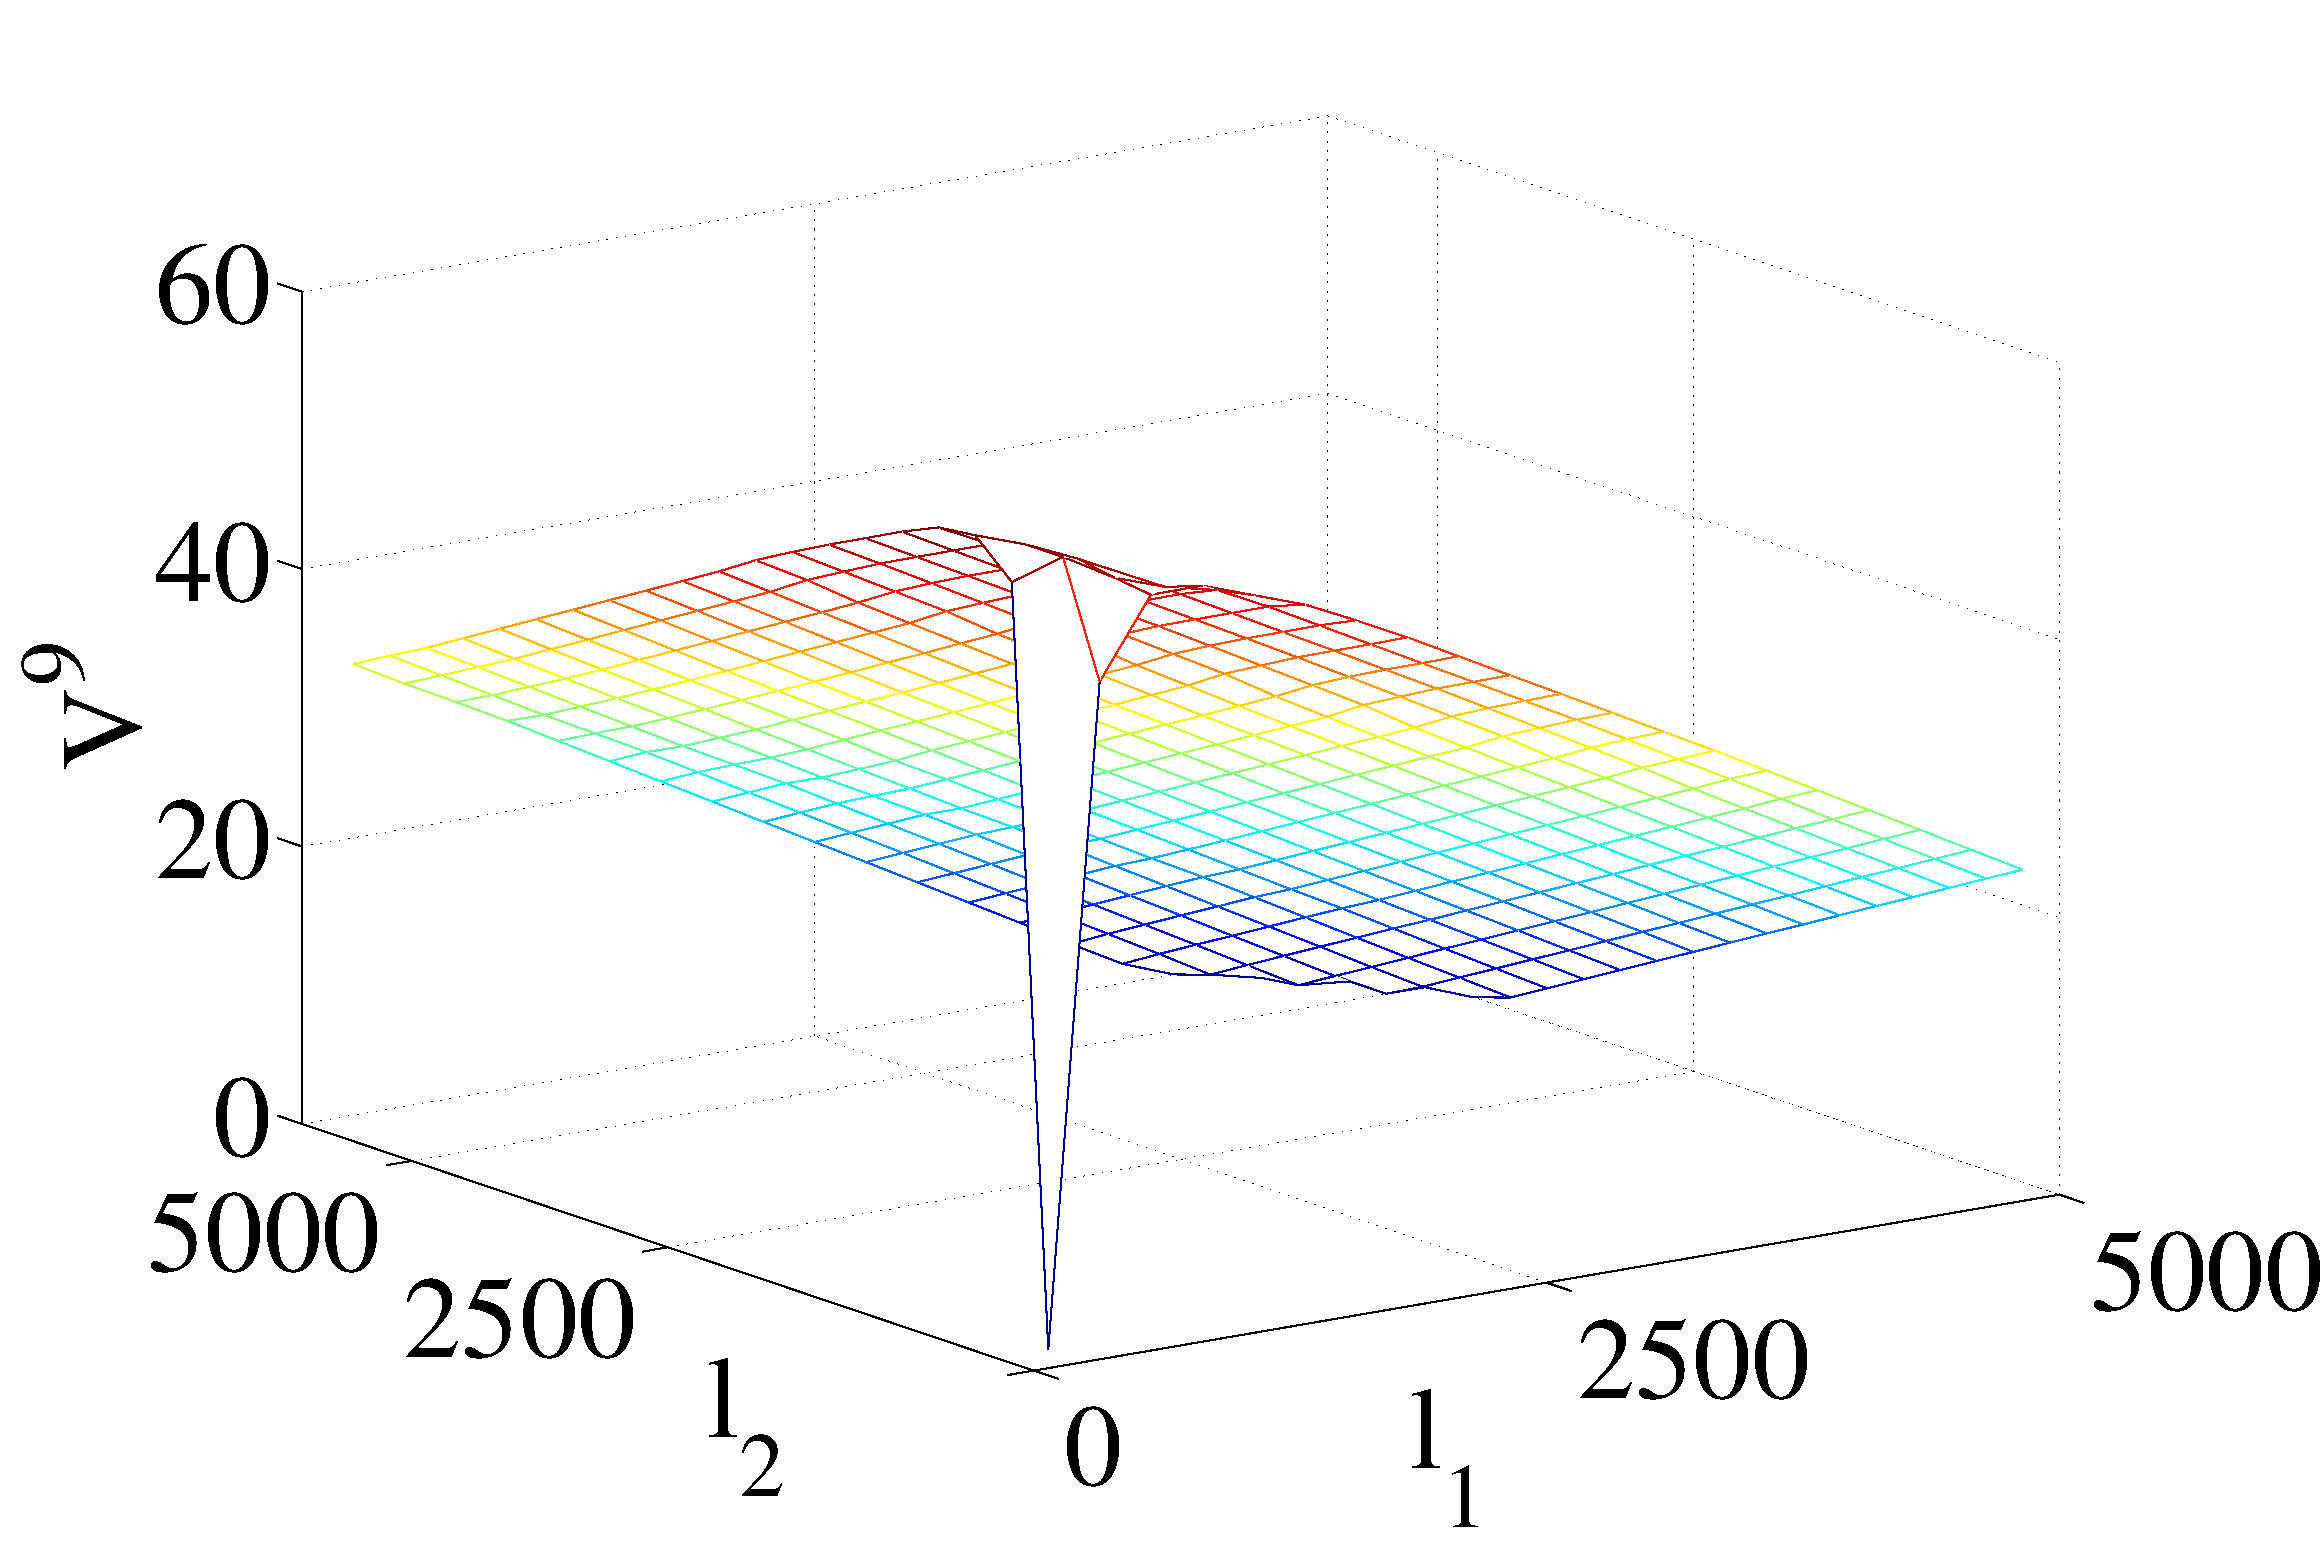
\includegraphics[width=0.3\textwidth]{new_pics/V9.pdf}
\vspace{-3mm}
\caption{\footnotesize 
\WaterReservoir: 
{\it (left)} Policy $\mathit{no}$-$\mathit{drain}(e)=\pi^{2,*}(l_1,l_2)$ 
for elapsed time $e$; 
{\it (middle)} $V^2(l_1,l_2)$; 
{\it (right)} $V^9(l_1,l_2)$.
}
\label{fig:v2plots}
\vspace{-4mm}
\end{figure*}
%%%%%%%%%%%%%%%%%%%%%%%%%%%%%%%%%%%%%%%%%%%%%%%%%%%%%%%%%%%%%%%%%%%%%%%%%% 

%%%%%%%%%%%%%%%%%%%%%%%%%%%%%%%%%%%%%%%%%%%%%%%%%%%%%%%%%%%%%%%%%%%%%%%%%%
% v9plot.pdf, Q-drain, Q-noDrain.pdf
%\begin{figure*}[t]
%\centering
%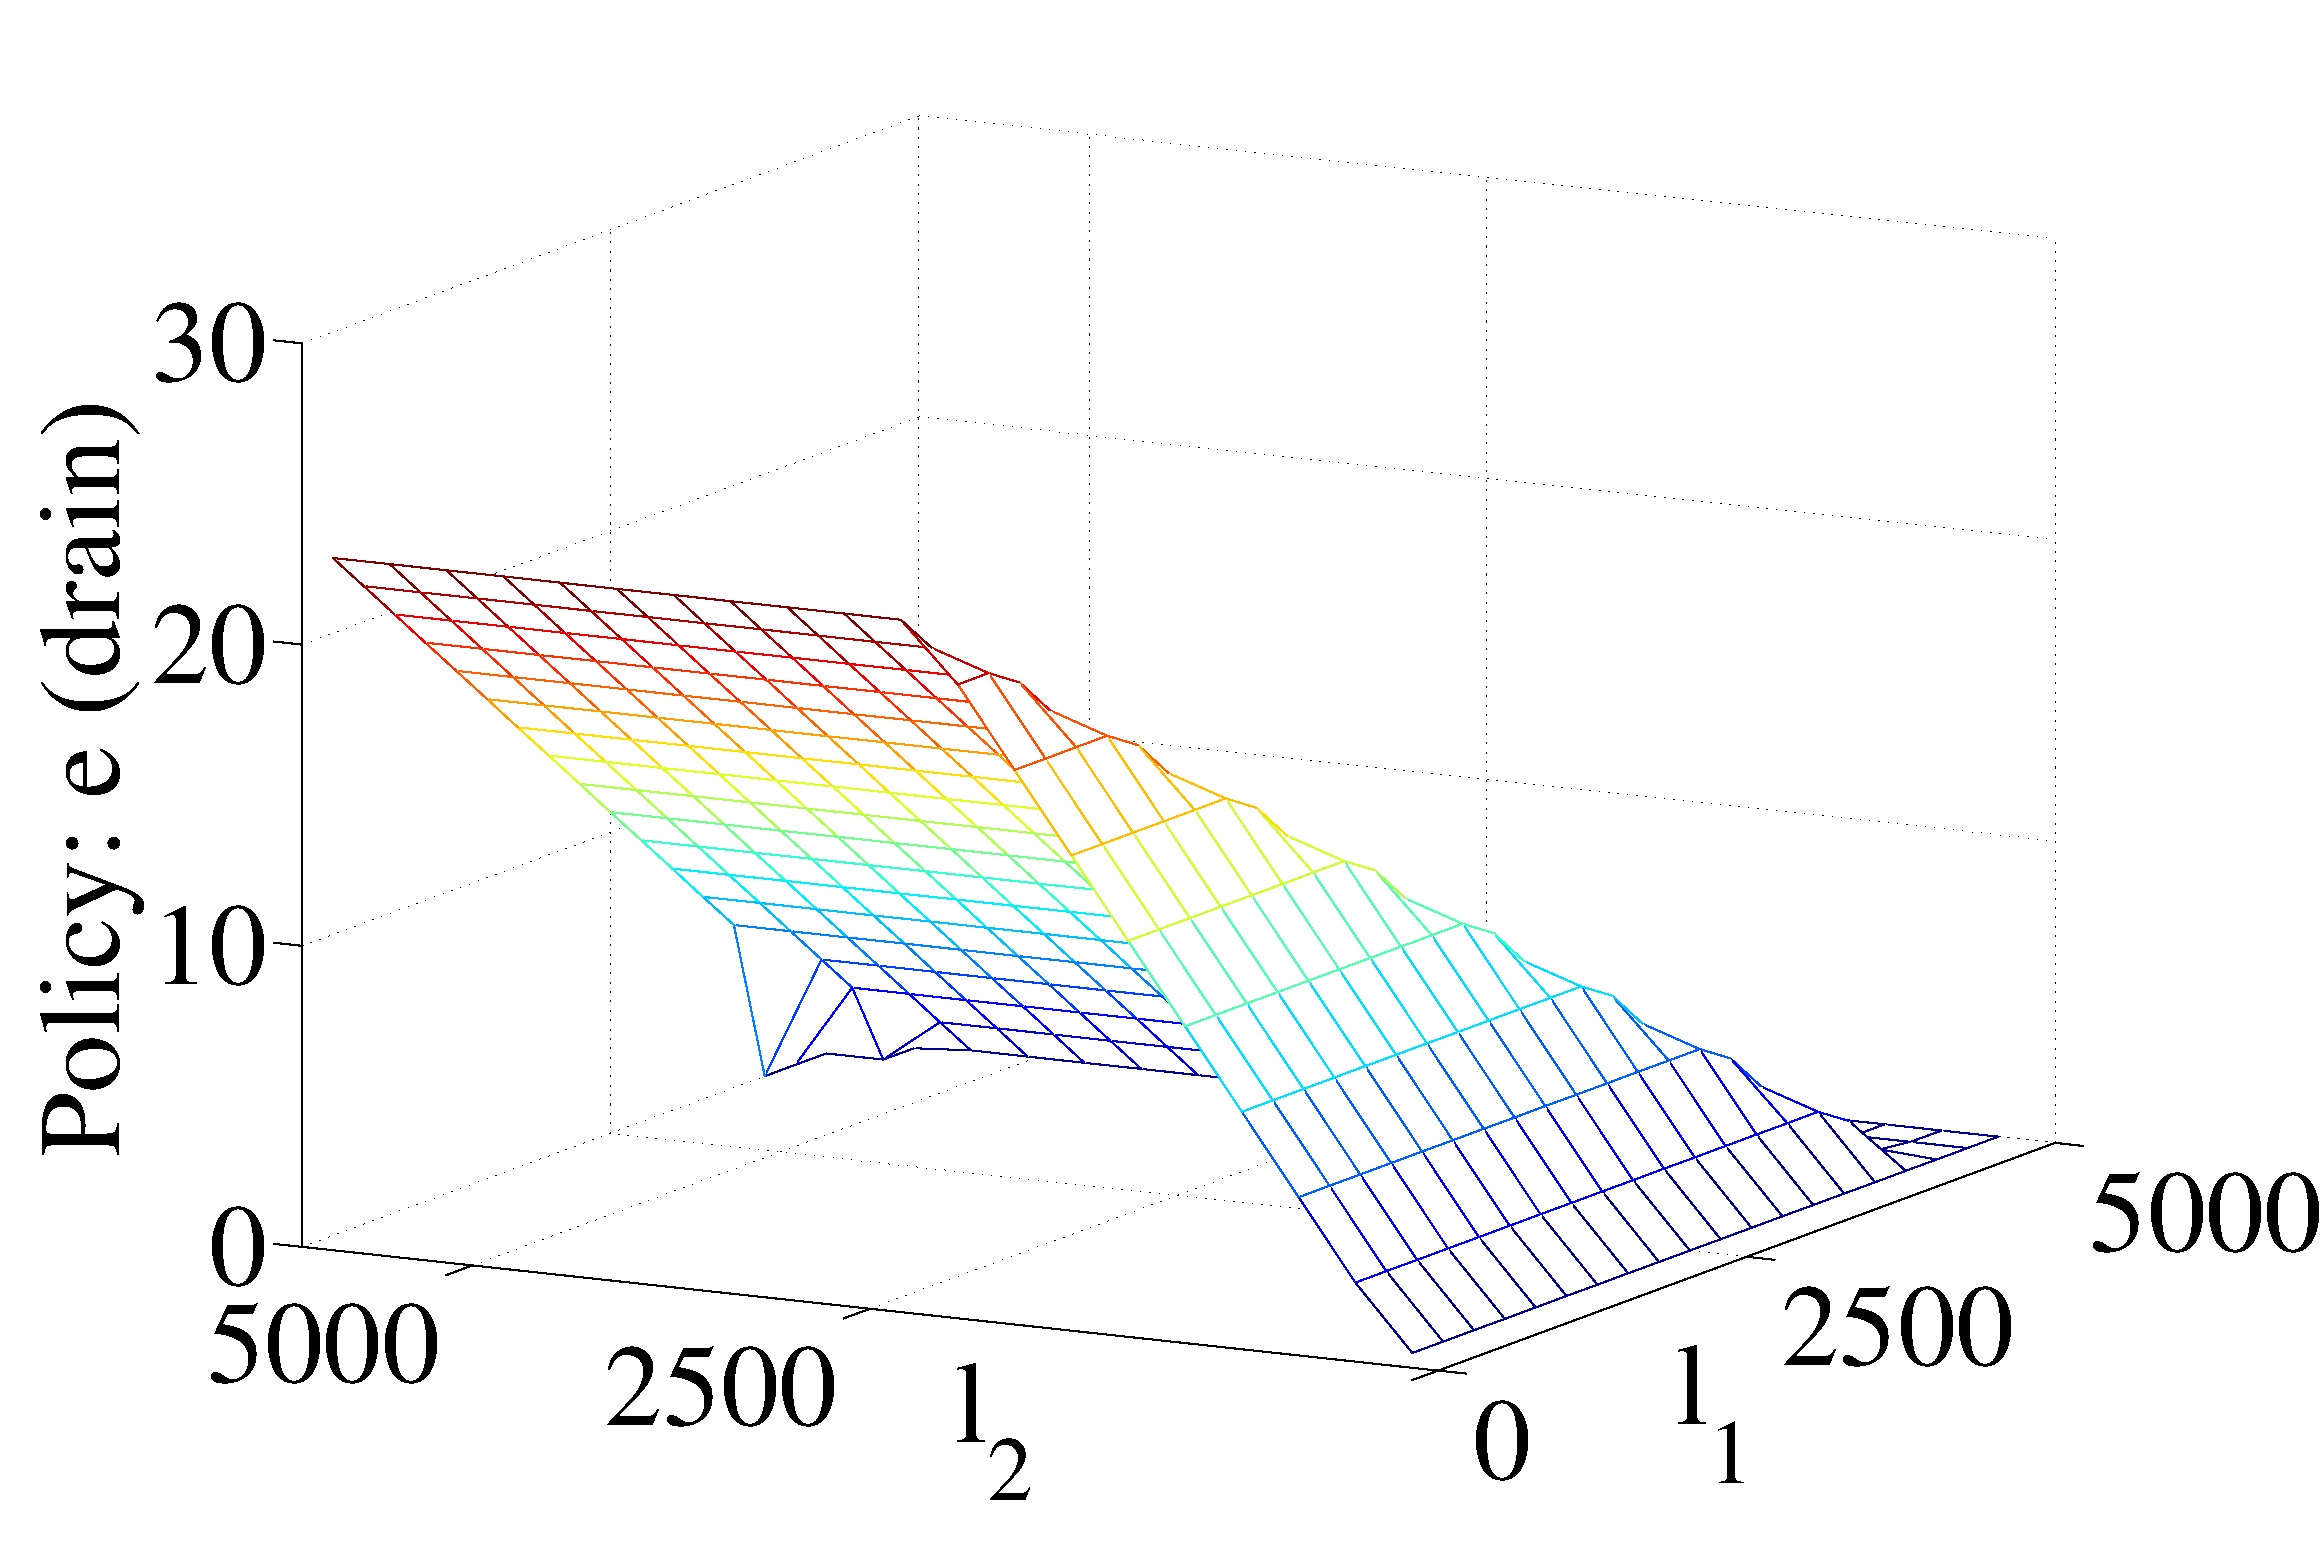
\includegraphics[width=0.33\textwidth]{new_pics/policy-iteration3-3.pdf}
%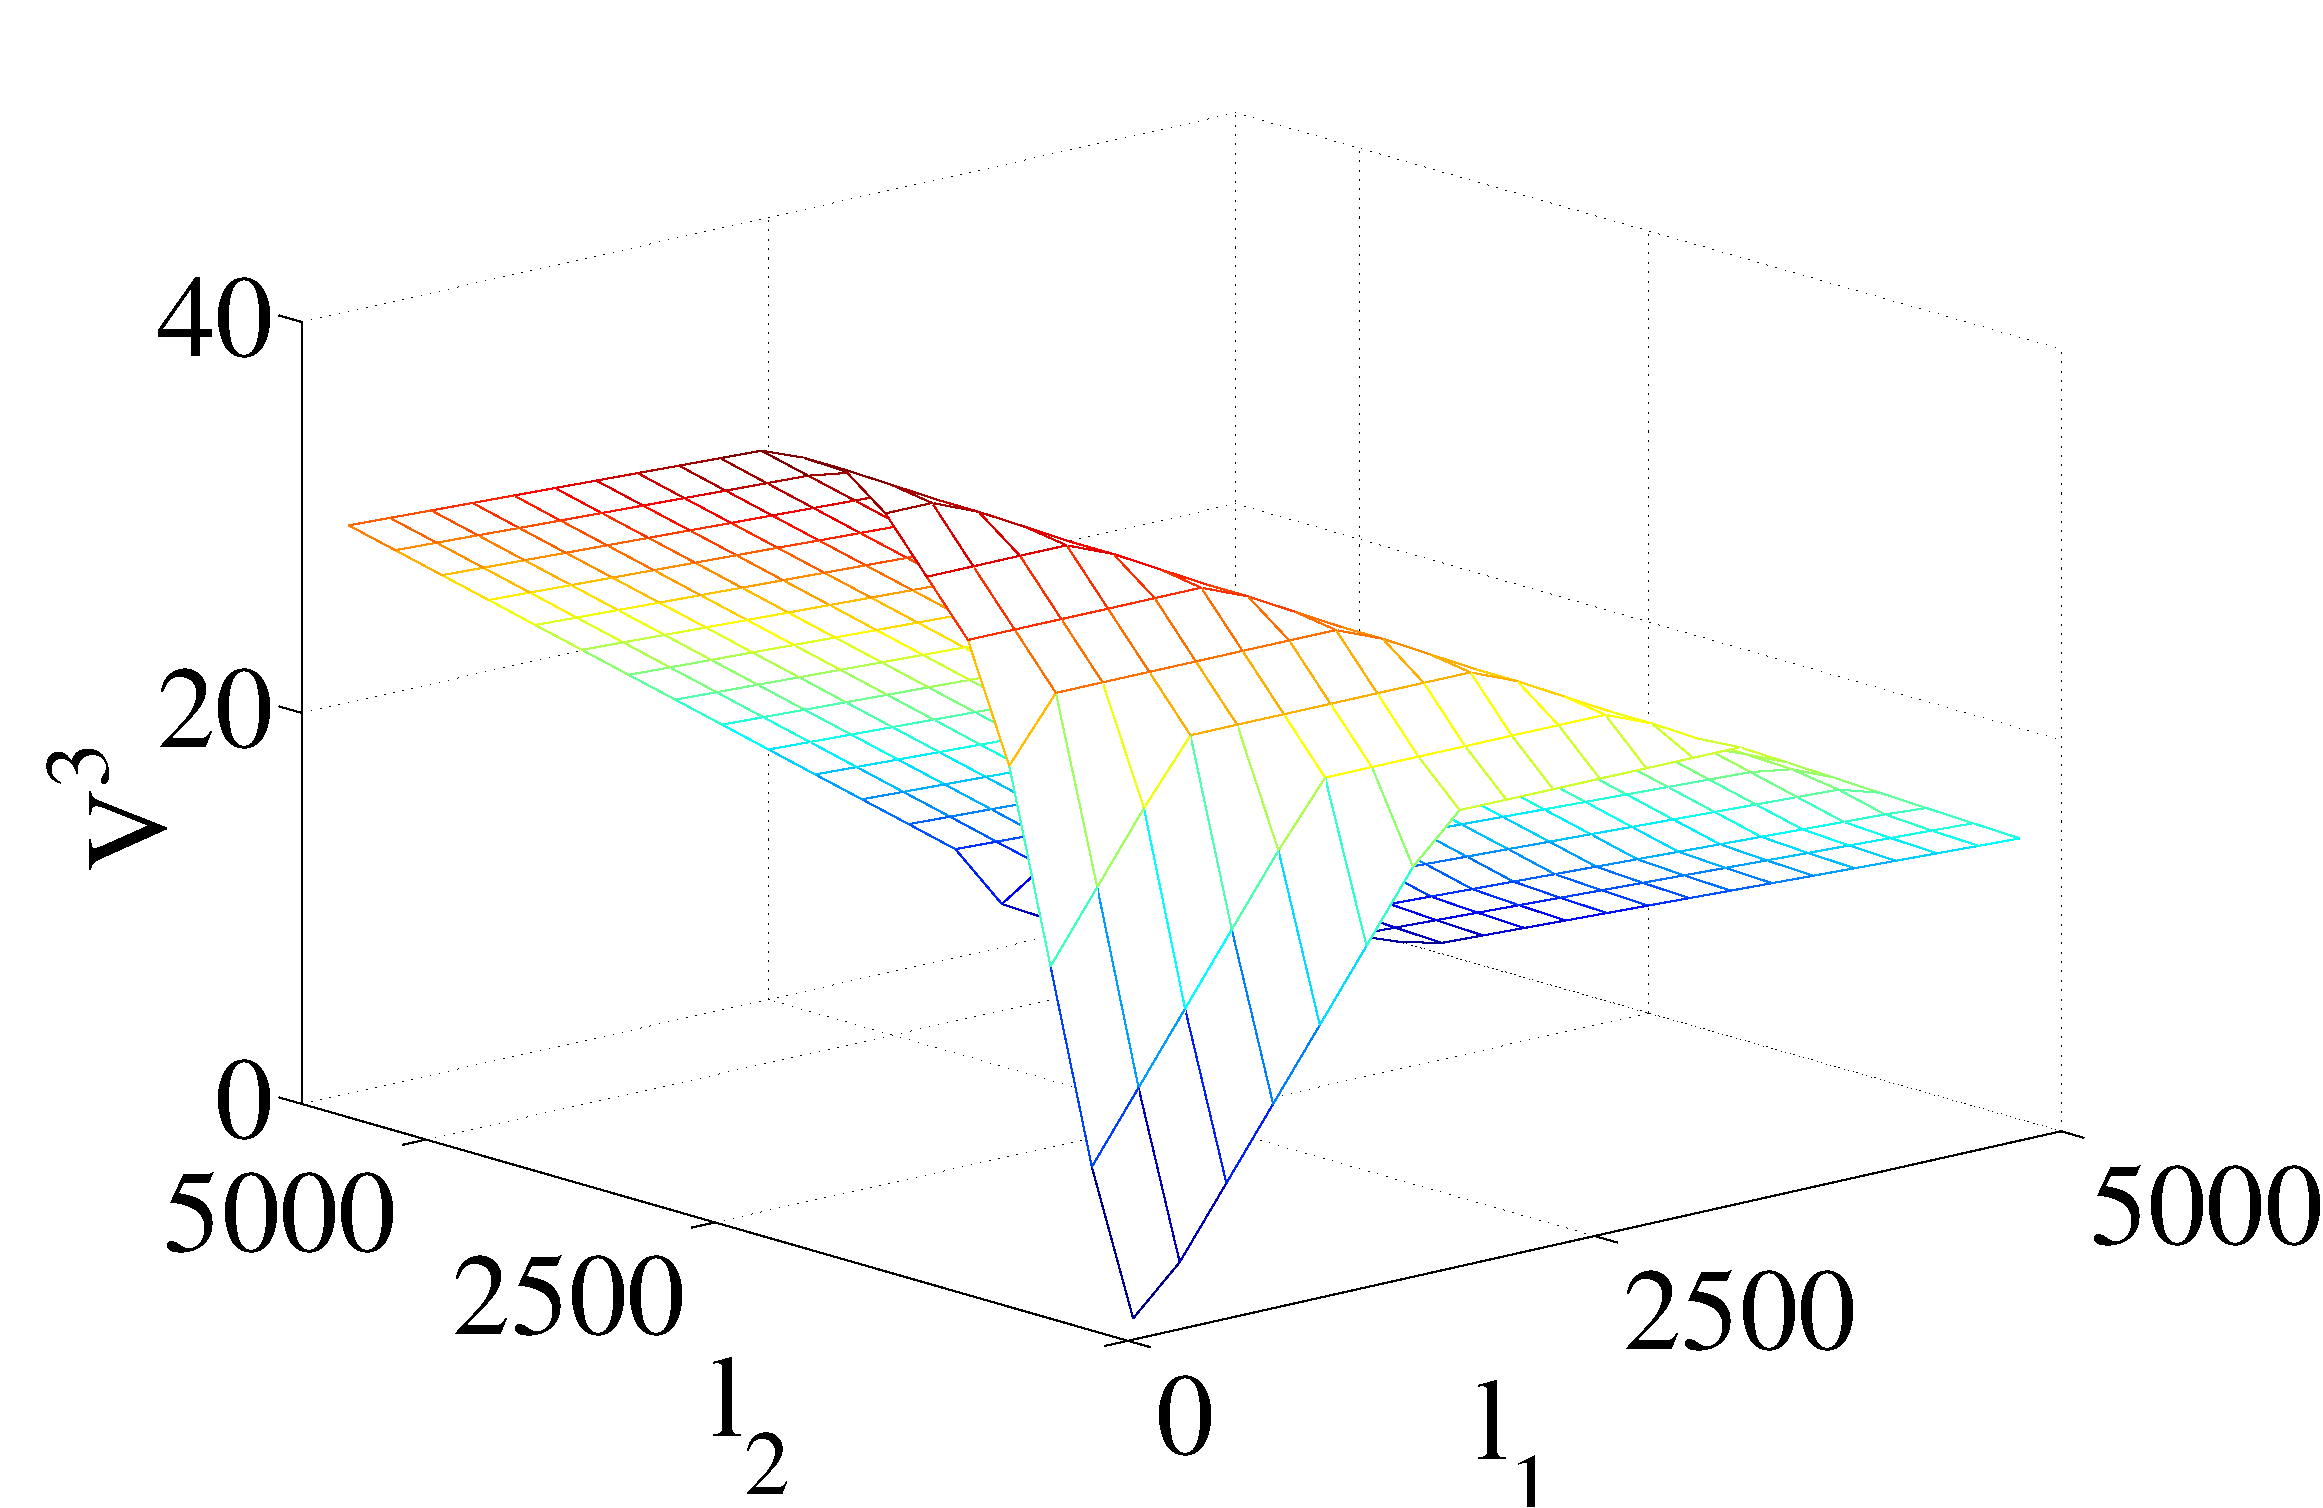
\includegraphics[width=0.33\textwidth]{new_pics/V3.pdf}
%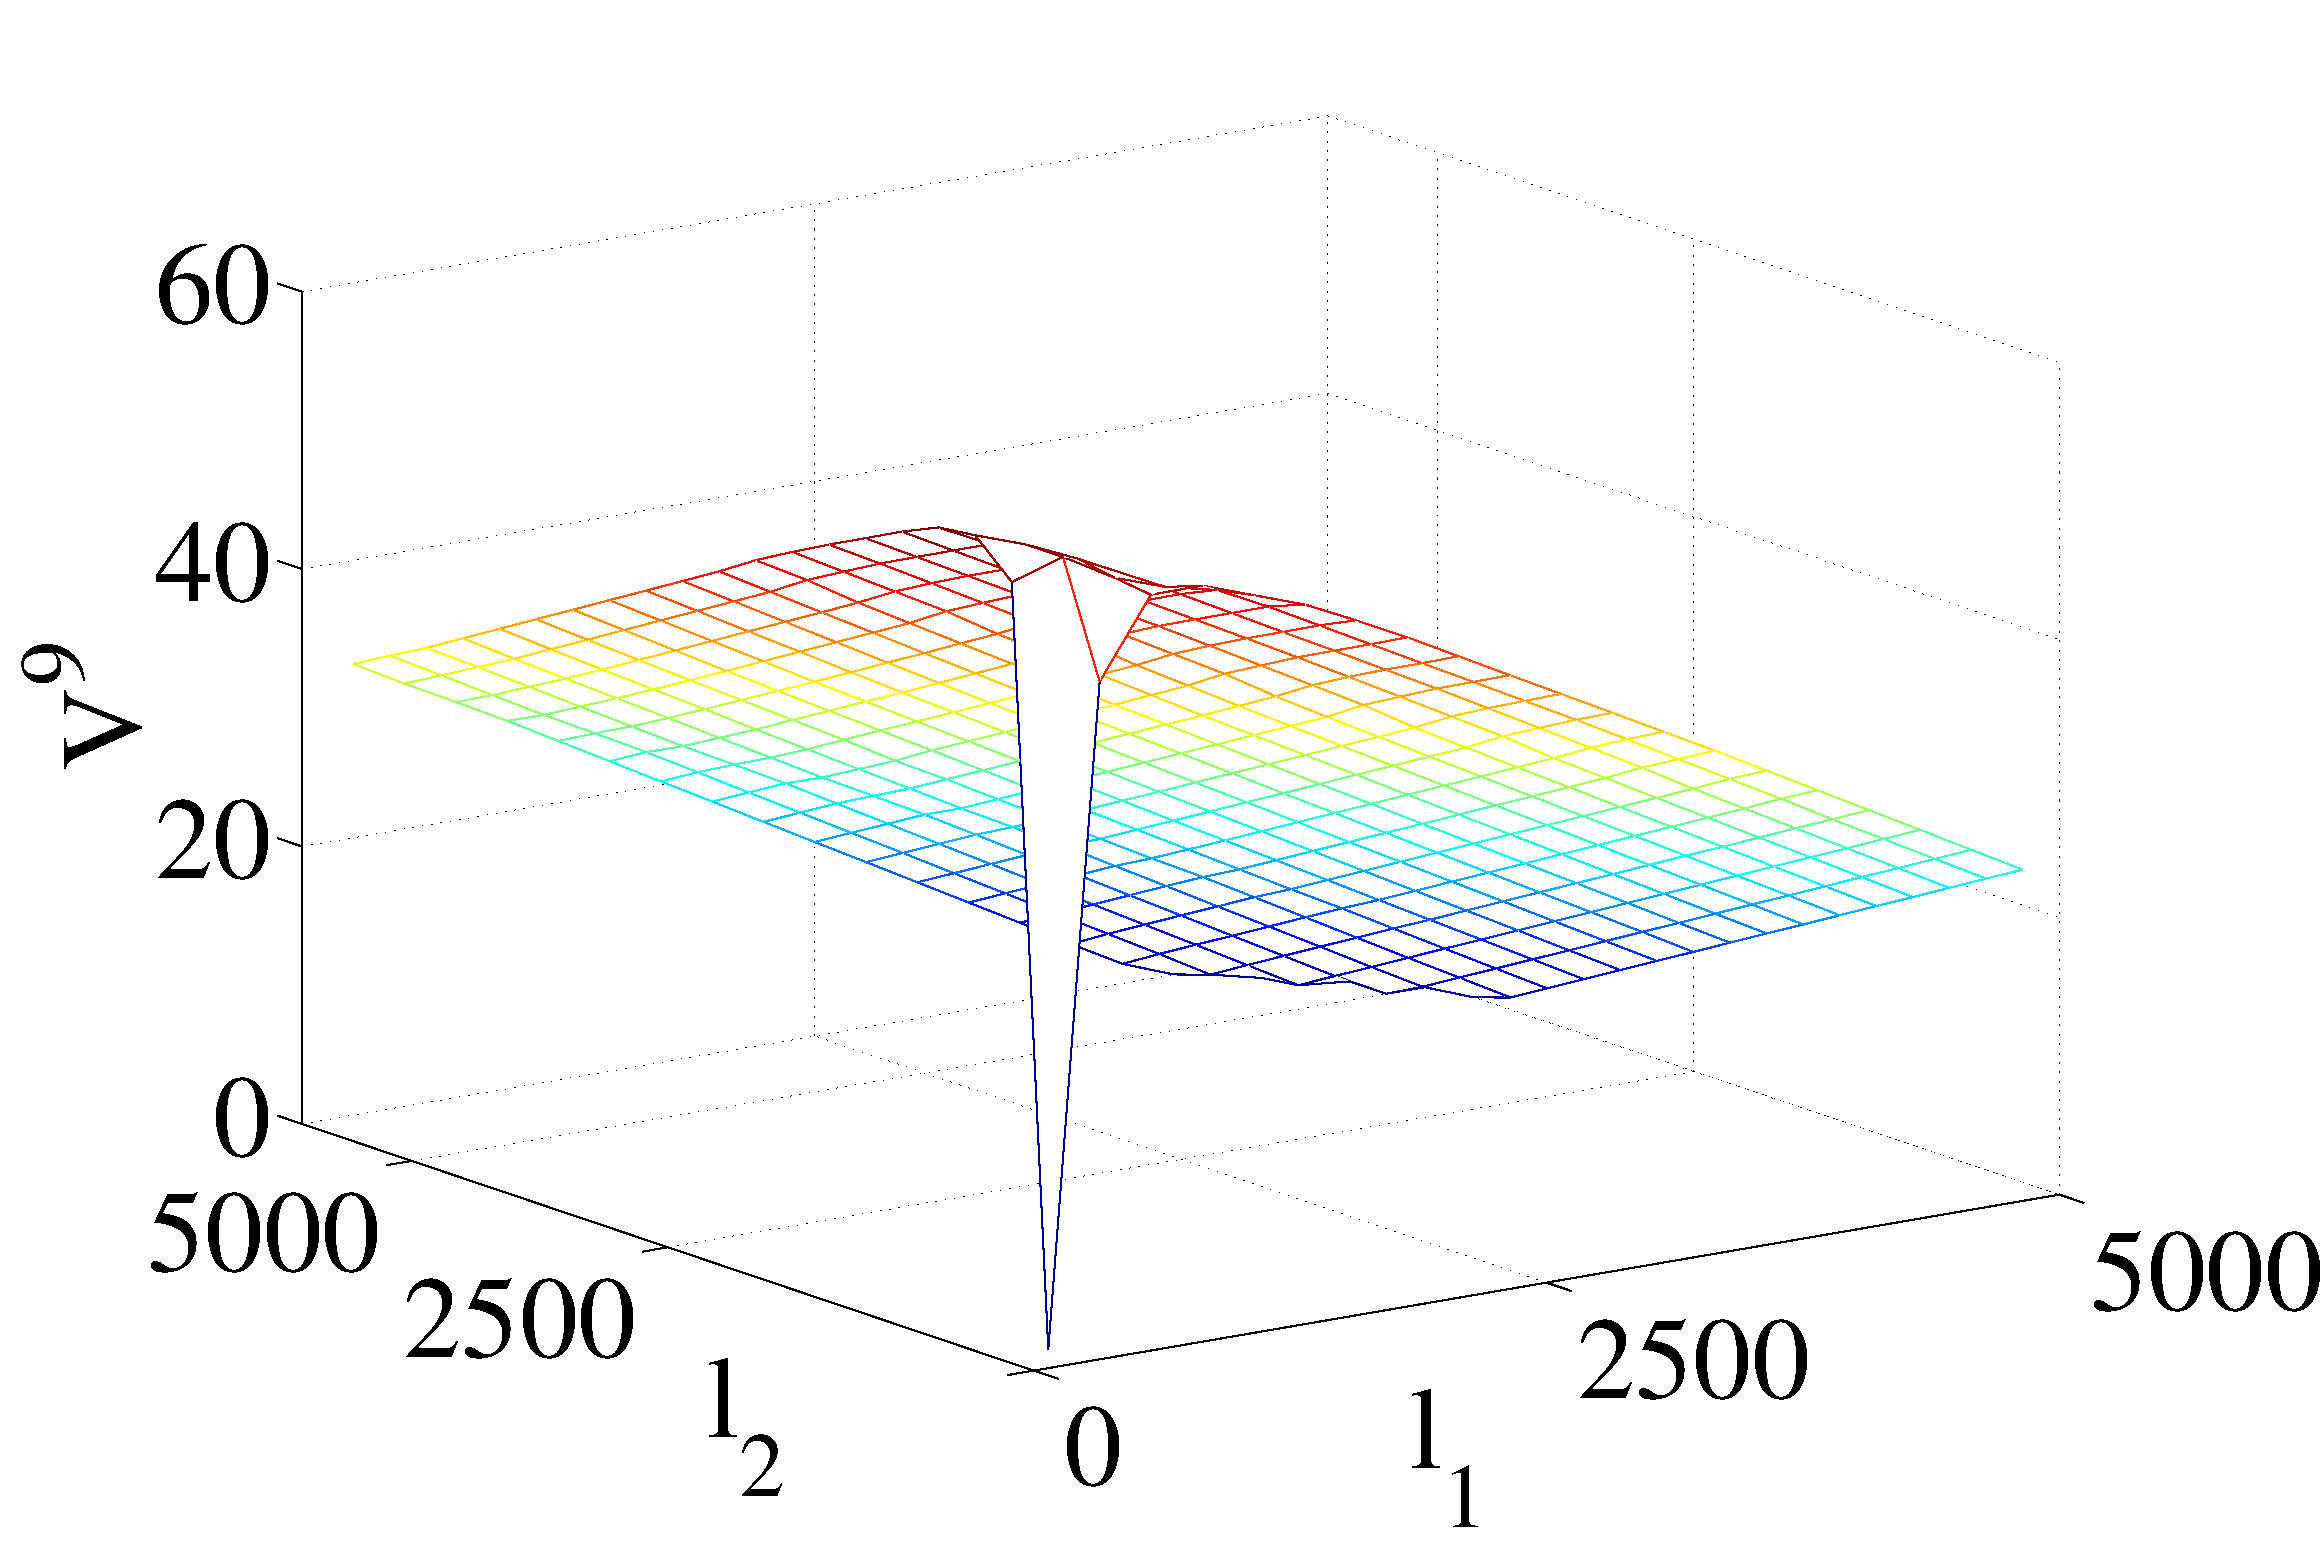
\includegraphics[width=0.33\textwidth]{new_pics/V9.pdf}
%\caption{%\footnotesize 
%Policy and Value of third iteration (Drain) and value of iteration 9.
%}
%\label{fig:v3plots}
%\vspace{-3mm}
%\end{figure*}
%%%%%%%%%%%%%%%%%%%%%%%%%%%%%%%%%%%%%%%%%%%%%%%%%%%%%%%%%%%%%%%%%%%%%%%%%% 

%%%%%%%%%%%%%%%%%%%%%%%%%%%%%%%%%%%%%%%%%%%%%%%%%%%%%%%%%%%%%%%%%%%%%%%%%%
%figure5 : time-iteration and space-iteraton for 1d-2d-noPrune inventory
\begin{figure}[tbp!]
\vspace{-2mm}
\centering
%\subfigure{
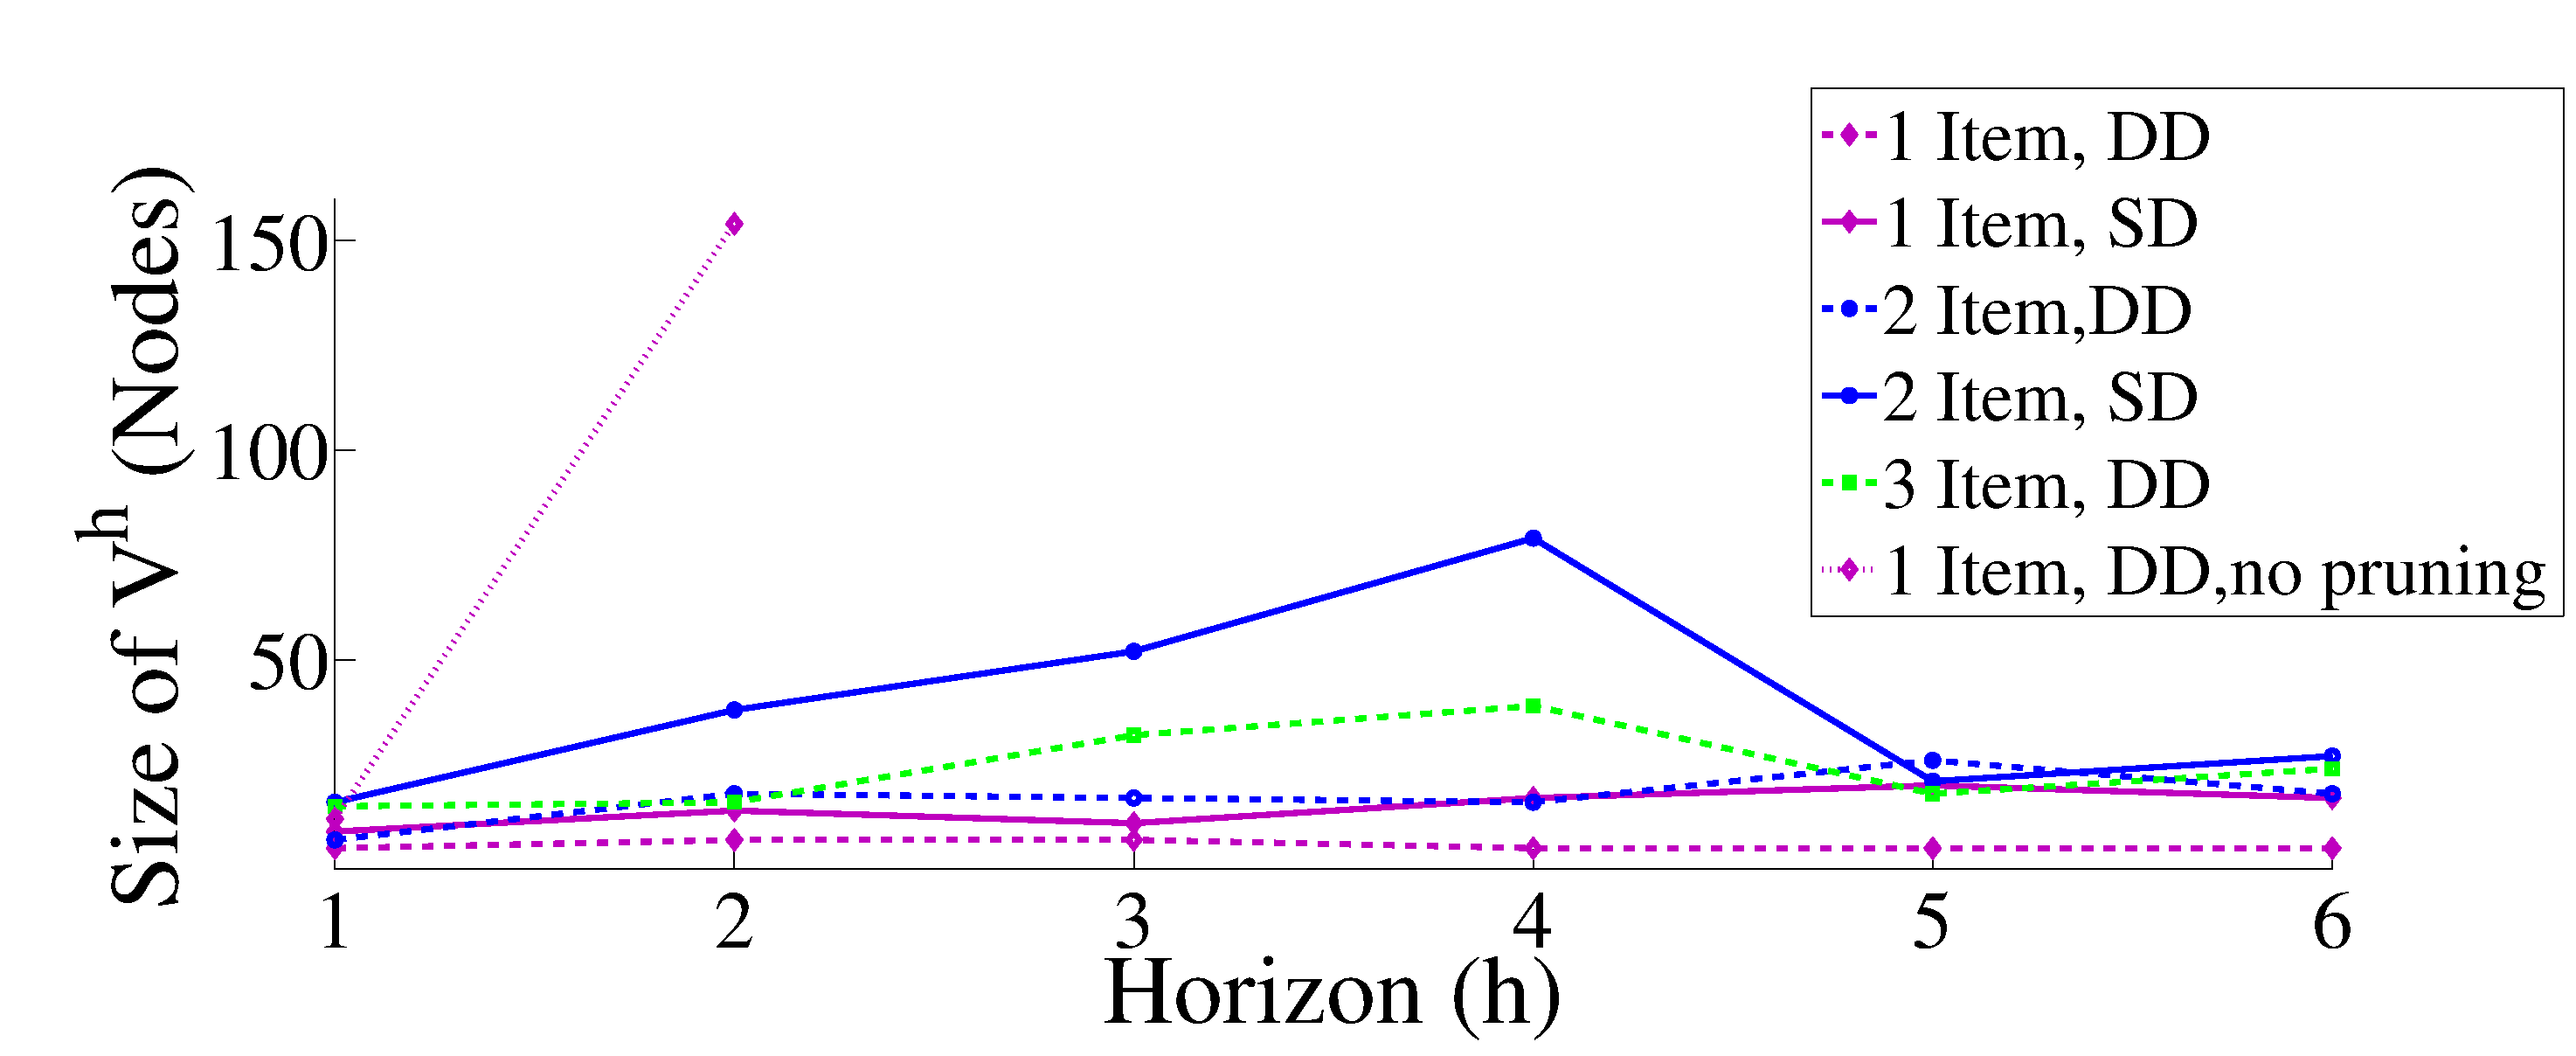
\includegraphics[width=0.42\textwidth]{new_pics/space1.pdf}\\
\vspace{-2mm}
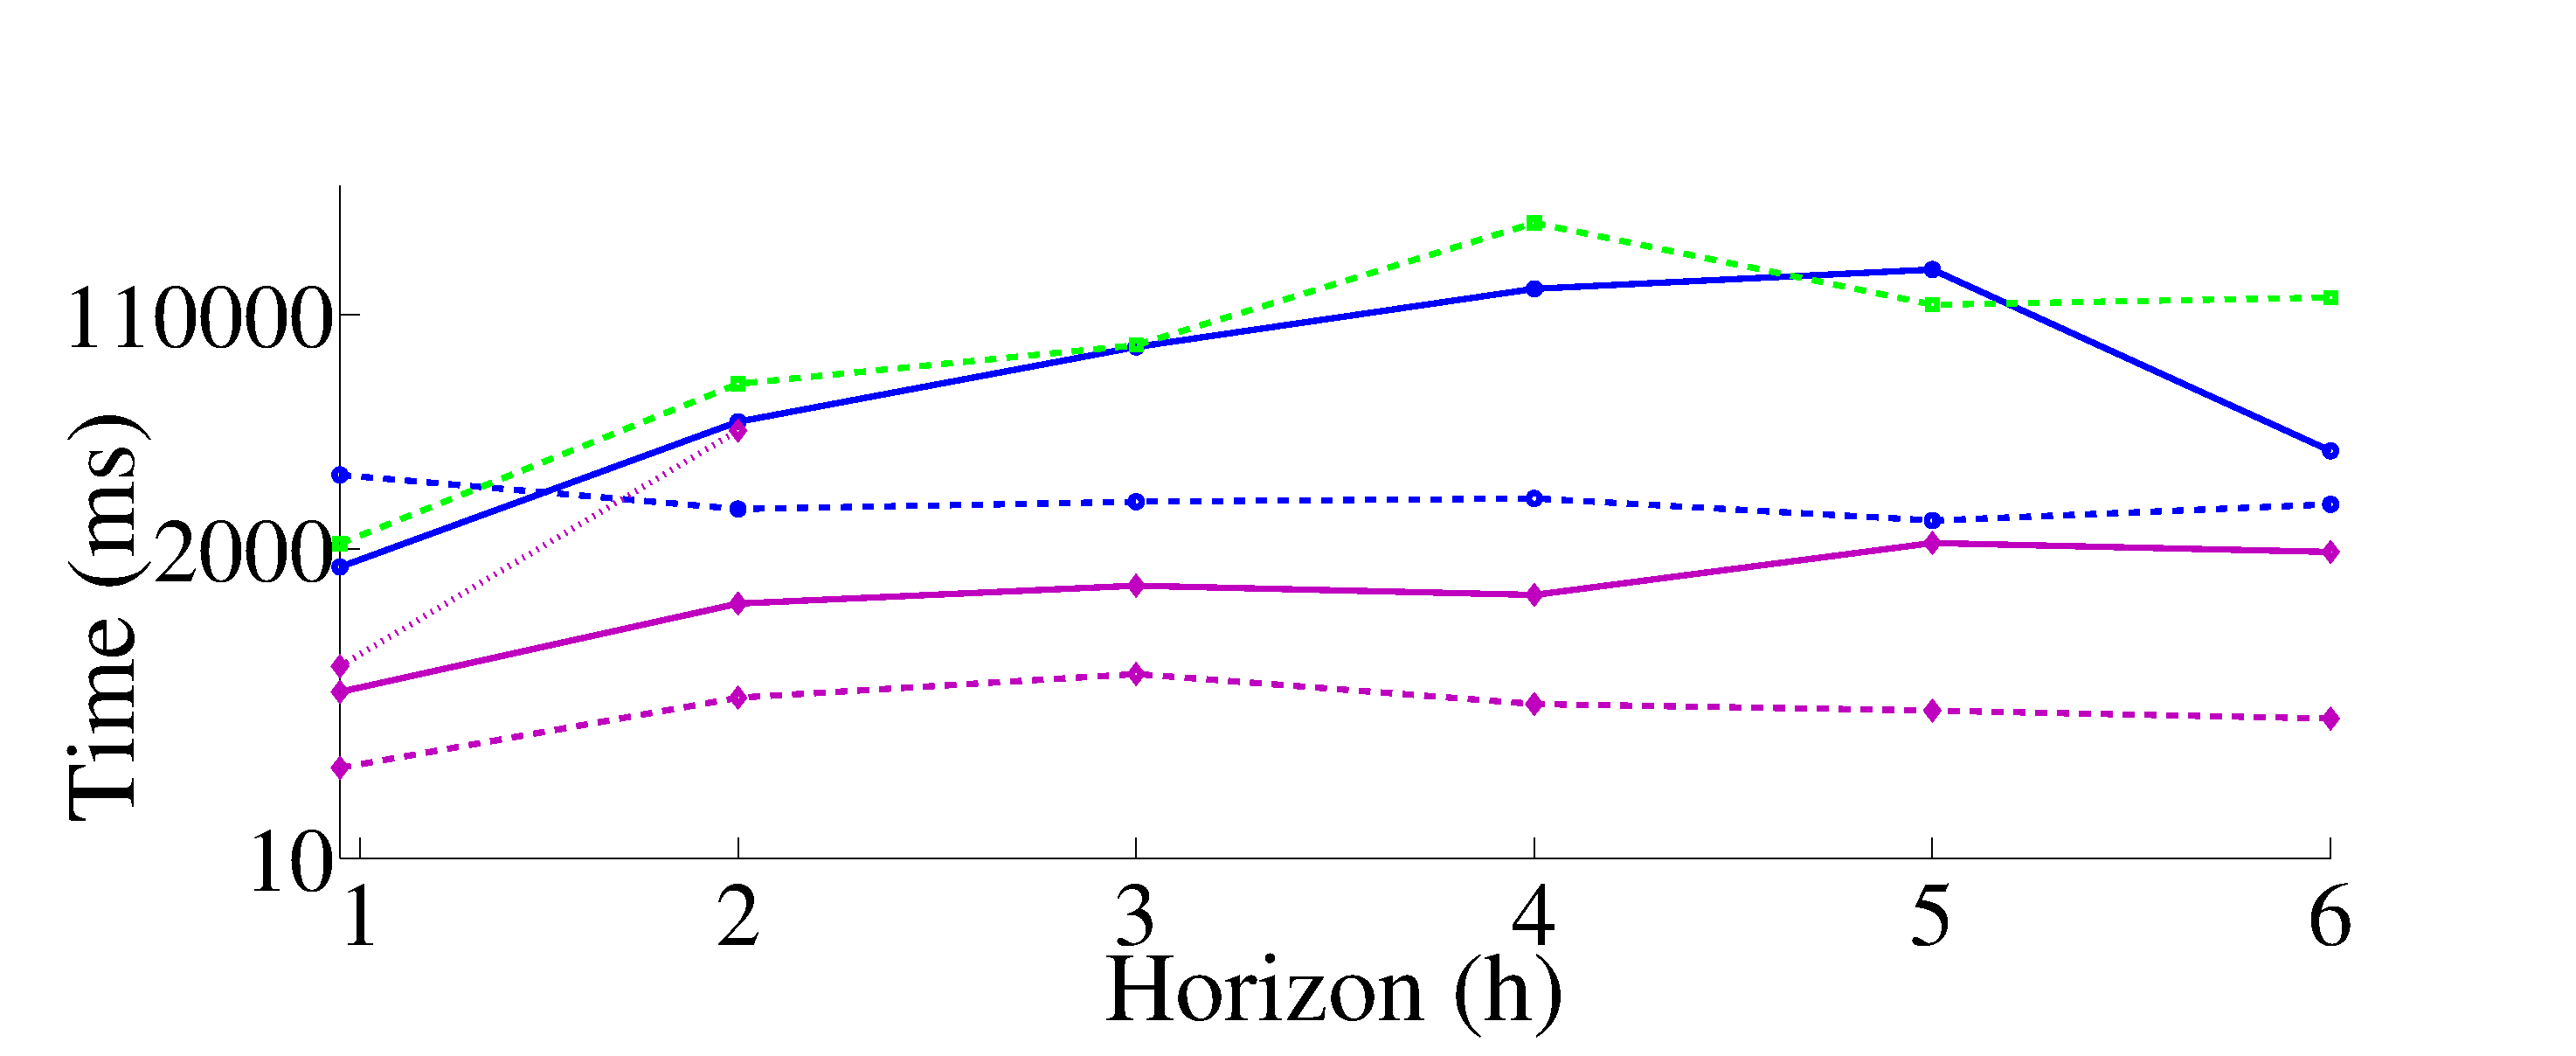
\includegraphics[width=0.42\textwidth]{new_pics/time1.pdf}
%}
\vspace{-2mm}
\caption{\footnotesize \InventoryControl: space 
and time vs. horizon.
% comparing 
%1,2 or 3 States and actions (SA) with Deterministic (DD) 
%or Stochastic (SD) demand and no-pruning}.
}
\label{fig:invC}
\vspace{-4mm}
\end{figure}
%%%%%%%%%%%%%%%%%%%%%%%%%%%%%%%%%%%%%%%%%%%%%%%%%%%%%%%%%%%%%%%%%%%%%%%%%%

\label{sec:results}
 
We evaluated SDP using XADDs on the didactic nonlinear
\MarsRover\ example and two problems from Operations Research (OR) --- 
\InventoryControl\ and \WaterReservoir --- described below.\footnote{
Full problem specifications and Java code to
reproduce these experiments are currently 
in Google Code; anonymity restrictions 
prevent us from providing this link in the submitted paper version.}
Space precludes showing 
more results for \MarsRover\ than in Figures~\ref{fig:opt_graph}
and~\ref{fig:opt_val_pol}; we note that SDP efficiently solves it
for arbitrary horizons.

{\bf \InventoryControl:} Inventory control problems (how much of an
item to reorder subject to capacity constraints, demand, and 
optimization criteria) date back to the 1950's with
Scarf's seminal optimal solution to the \emph{single-item capacitated
inventory control} (SCIC) problem~\cite{Scarf_Karlin58}.
\emph{Multi-item joint capacitated inventory} (MJCIC) control (upper limits
on total storage of all items) has proved to be an NP-hard problem and
as a consequence, most solutions resort to some form of
approximation~\cite{bitran,wusd10}; indeed, we are unaware of any 
work which claims to find an exact closed-form non-myopic
optimal policy for \emph{all} (continuous) inventory states for MJCIC 
under linear reordering costs and linear holding costs; these 
problems can be easily modeled as CSA-MDPs and solved optimally
with SDP.  

In Figure~\ref{fig:invC}, we provide a time and space analysis of
deterministic- and stochastic-demand (resp. DD and SD) variants of the
SCIC and MJCIC problem for up to three items (the same scale of
problems often studied in the OR literature); for each number of items
$n \in \{ 1,2,3 \}$ the state (inventory levels) is $\vec{x} \in
[0,\infty]^n$ and the action (reorder amounts) is $\vec{y} \in
[0,\infty]^n$.  Orders are made at one month intervals and we solve
for a horizon up to $h=6$ months.  Here we see that linear feasbility
checking/pruning in the XADD is crucial -- we cannot solve beyond
$h=2$ without it for 1 item!  While solving for larger numbers of
items and SD (rather than DD) both increase time and space, 
the solutions quickly reach quiescence indicating structural
convergence.

%{\footnotesize
%\begin{align*}
%x'_1 & = \begin{cases}
%d \wedge (x_1 + a_1 - 150 \leq 200) : & x_1 + a_1 - 150 \\
%d \wedge (x_1 + a_1 - 150 \geq 200) : & x_1 - 150 \\
%\neg d \wedge (x_1 + a_1 - 50 \leq 200): & x_1 + a_1 - 50 \\
%\neg d \wedge (x_1 + a_1 - 50 \geq 200): & x_1 - 50 \\
%\end{cases}
%\end{align*}}

{\bf \WaterReservoir:} Reservoir management is also well-studied in
OR~\cite{Mahootchi2009,Yeh1985}.  The key continuous decision is how
much elapsed time $e$ to
\emph{drain} (or \emph{not drain}) each reservoir to maximize
electricity revenue over the decision-stage horizon while avoiding
reservoir overflow and underflow.  Cast as a CSA-MDP, we 
believe SDP provides the first approach capable of deriving
an exact closed-form non-myopic optimal policy
for all levels.

We examine a 2-reservoir problem with
respective levels $(l_1,l_2)\in [0,\infty]^2$ with reward penalties for 
overflow and underflow and a reward gain linear in the elapsed time $e$ for
electricity generated in periods when the $\mathit{drain}(e)$ action
drains water from $l_2$ to $l_1$ (the other action is 
$\mathit{no}$-$\mathit{drain}(e)$); we assume deterministic rainfall
replenishment.  In Figure~\ref{fig:v2plots}, we show a plot of 
the optimal closed-form policy
at $h=2$: the solution interleaves $\mathit{drain}(e)$ and 
$\mathit{no}$-$\mathit{drain}(e)$ where even horizons are the latter;
here we see that we avoid draining for the longest elapsed time $e$ 
when $l_2$ is low (wait for rain to replenish) and $l_1$ is high (draining
water into it could overflow it).  $V^2(l_1,l_2)$ and $V^9(l_1,l_2)$
show the progression of convergence from horizon $h=2$ to $h=9$ ---
low levels of $l_1$ and $l_2$ allow the system to generate electricity
for the longest total elapsed time over 9 decision stages.


% or put complete description here: 
%The transition function is demonstrated below: 
%{\footnotesize
%\begin{align*}
%l_1'  = 400 * e + l_1 -700 * e + 500 * e \\
%l_2'  = 400 * e + l_2 - 500 * e \\
%\end{align*}
%}

%Here we take draining as the act of discharging water levels per
%time-step from the upper-stream reservoir to the down-stream reservoir
%($500 * e$). A constant amount of discharge is always considered for
%the down-stream to ensure all electricity demands are fulfilled.  The
%amount of rain (r) is considered as a constant which affects both
%reservoirs at the time of discharge.

%The reward function for both actions considers the safe range of
%[50,4500] as the safe water levels and assigns a positive reward of
%$e$ for the action of draining, and no rewards ( but also no penalty)
%for not draining. If the next state is not in the safe range, a huge
%penalty of -1+e6 is assigned as the reward.
%
%{\footnotesize
%\begin{align*}
%(l_1\leq 4500 - 200 * e) \wedge (l_2 \leq 4500 +100 *e) \\
%\wedge (l_1\geq 50 - 200 * e) \wedge (l_2 \geq 50 +100 *e) : e \\
%\end{align*}
%}
